% Szglab4
% ===========================================================================
%
\chapter{Követelmény, projekt, funkcionalitás}

\thispagestyle{fancy}

\section{Bevezetés}

\subsection{Cél}

A dokumentum célja az elkészülendő szoftver bemutatása fejlesztői szemszögből, ami a szoftver fejlesztői dokumentációja, amely segítségével megismerhető a szoftver felépítése és fejlesztésének lépései.
%\comment{A dokumentum célja.}

\subsection{Szakterület}

A kialakítandó szoftver egy játék, amely kizárólag szórakoztatási célokat szolgál. A fejlesztők célja egy olyan szoftver létrehozása, amely megfelel a feladatkiírásban foglalt követelményeknek.
%\comment{A kialakítandó szoftver milyen területen használható, milyen célra.}

\subsection{Definíciók, rövidítések}
\begin{description}
\item[HSZK] Hallgatói Számítógép Központ
\item[szoftver] a program amit írunk
\end{description}


%\comment{A dokumentumban használt definíciók, rövidítések magyarázata.}

\subsection{Hivatkozások}

\begin{itemize}
\item \url{http://en.wikipedia.org/wiki/Tower_defense}
\item \url{http://en.wikipedia.org/wiki/The_Lord_of_the_Rings_(film_series)}
\end{itemize}

%\comment{A dokumentumban használt anyagok, web-oldalak felsorolása}

\subsection{Összefoglalás}

A dokumentum további részei az analízis modell, ami a szoftver főbb osztályainak, alkotóelemeinek tárgyalása, a szkeleton, amiben a belső működést tárgyaljuk.

A prototípus részben a részletes terveket, use-case-eket lehet majd megtalálni.

A szoftver grafikus tulajdonságait, interfészét, a végső fázisban dokumentáljuk.



%\comment{A dokumentum további részeinek rövid ismertetése}

\section{Áttekintés}
\subsection{Általános áttekintés}
A szoftver kialakítandó architektúrája objektum-orientált, modell-nézet-vezérlő mintát követ.

A modell fontosabb alrendszerei:%
\begin{itemize}
\item pálya, 
\item tornyok, 
\item akadályok, 
\item ellenségek.
\end{itemize} 
	 
Az ellenségek, illetve a tornyok és akadályok közötti kapcsolat lényege, hogy a tornyok tudják, mikor ér a hatókörükbe egy ellenség. A tornyoknak tudniuk kell értesíteni az ellenségeket, amikor tüzet nyitnak, ami alapján az ellenségnek változik az életereje.
 
A pálya és az ellenségek közötti kapcsolat lényege, hogy az ellenségek ismerjék a pályán lévő utat, tudják azt követni.

%\comment{A kialakítandó szoftver legmagasabb szintű architekturális képe. A fontosabb alrendszerek felsorolása, a közöttük kialakítandó interfészek lényege, a felhasználói kapcsolatok alapja. Esetleges hálózati és adattárolási elvárások.}

\subsection{Funkciók}
\subsubsection{Az eredeti feladatkiírás szövege} 

A gonosz emberek, tündék, törpök és hobbitok szövetséget kötnek, hogy elpusztítsák az Egy Gyűrűt a Végzet Hegyénél. Szerencsére csak Mordor földjén keresztül tudnak eljutni a hegyhez, így jóságos Szarumánnak lehetősége van védelmi tornyokat építeni, hogy segítsen megvédeni Szauron hatalmát. A játék célja annak megakadályozása, hogy a Gyűrű szövetségének tagjai közül bárki is eljusson a Végzet Hegyéhez. Egy ellenség akkor pusztul el, ha összességében megfelelő mértékű sebzést kap a tornyokból származó lövedékektől. A tornyok építéséhez Szarumánnak a varázserejét kell használnia. Szarumán akkor tud tornyot építeni, ha megfelelő mennyiségű varázsereje van hozzá. A varázsereje minden egyes elpusztított ember, tünde, törp vagy hobbit után bizonyos mértékben növekszik.

A Gyűrű szövetségének tagjai különböző utakon juthatnak el a Végzet Hegyéhez. Az utakról nem térhetnek le. Szarumán az utakra nem tud tornyot építeni, csak az utak mellé. Az utakra azonban tehet akadályokat, amik az akadály területén lassítják az ellenség haladását. A tornyoknak van egy adott hatótávolsága és tüzelési gyakorisága. Szarumán a varázserejét arra is használhatja, hogy a tornyokat és akadályokat különböző varázskövekkel ruházza fel. A varázsköveknek több fajtája is létezik, és különböző hatásúak lehetnek. Egyes kövek növelhetik a tornyok hatótávolságát vagy tüzelési gyakoriságát, más kövek egy-egy típusú ellenfél esetén megnövelik a lövedékek sebzési erejét.

A játék során az ellenségek folyamatosan jönnek. A játék elején ritkábban, később gyakrabban és nagyobb csoportokban, azonban számuk véges, előbb-utóbb elfogynak. A játék akkor ér véget, ha egy ellenség eljut a Végzet Hegyéhez, vagy ha már sikerült az összes ellenséget kiirtani. Az első esetben Szauron és Szarumán megsemmisül, utóbbi esetben fényes győzelmet aratnak, és örökké uralni fogják a világot.

\subsubsection{Feladat specifikációja}

A feladat egy grafikus felületű logikai játékszoftver készítése Java nyelven, ami megfelel a fenti leírás szövegének, továbbá működik a HSzK számítógépein. 

A szoftver elindítása után a kezdőképernyő fogadja a felhasználót, ahol új játékot indíthat a megfelelő gombbal. Az új játék indítása esetén a felhasználónak ki kell választania egy pályát. Ha ez megtörtént, elindul a játék. 

A pályák téglalap alakúak és különböző méretűek lehetnek. A pályák egy n*m méretű négyzetrácsból állnak, ahol m a sorok n pedig az oszlopok számát jelenti. 

A pálya négyzetrácsos szerkezetének a celláira a játékos védelmi egységeket helyezhet varázserőért cserébe. A cellák két típusúak lehetnek: út, és háttér. A hátteret alkotó cellákra tornyokat lehet helyezni, az út celláira pedig akadályokat. 

A tornyoknak 	három jellemzője van: tüzelési sebesség, sebzés és hatótáv. Amint egy ellenség egy torony hatókörébe ér, az tüzet nyit rá, azonban egy torony egyszerre csak egy célpontra tüzelhet. Lehetséges a tornyokat fejleszteni is: két hely van minden toronyban, amibe a torony további képességeit, azaz a hatótávolságot és a tüzelési gyorsaságot fokozó kristályokat helyezhetünk. Végül pedig minden torony esetén lehetőség van egy darab, az egyes fajok elleni sebzést növelő kristályt helyezni.

Az út celláira elhelyezhető akadályok lassítják a felettük elhaladó ellenségeket, viszont elhelyezésük után használódnak minden ellenség lassításakor, míg végül meg nem szűnnek. Az akadályok jellemzői, hogy mennyi ellenség haladhat át rajtuk és a lassítás mértéke. Az akadályokat is lehetséges fejleszteni: lehet növelni a lassítás mértékét, illetve meg lehet javítani az akadályt. 

A tornyok és akadályok elhelyezése úgy történik, hogy a játékos a kívánt cellára kattint, majd a felkínált lehetőségek közül kiválasztja az elhelyezendő tornyot, illetve akadályt. 

A védelmi egységeket el is adhatja a játékos, ekkor az arra fordított varázserőnek, tehát a vásárlás és az esetleges fejlesztések árának a fele visszatérül. Az eladásához először rá kell kattintani az eladni kívánt védelmi egység képére, majd a megjelenő lehetőségek közül ki kell választani az eladást. Az akadályok esetén a visszajáró varázserő az elhasználtság mértékétől is függ: a ráfordított költségek felét, tehát ami egy torony esetén visszajárna, még meg kell szorozni az ellenségek számának, amik még áthaladhatnak az akadályon, és az ellenségek számának, amik összesen áthaladhatnak az akadályon, hányadosával.
 
A tornyok és akadályok fejlesztéséhez a felhasználó kiválasztja a fejleszteni kívánt egységet a rajta való kattintással, és megjelennek az azzal kapcsolatos műveletek, amelyek között szerepel az egység különböző módú fejlesztése is. Minden fejlesztés varázserőbe kerül. 

Egy ellenségnek két jellemzője van: a sebessége és az életereje. A játékban négy különböző ellenfél van: emberek, tündék, törpök és hobbitok. Minden fajnak különböző jellemzőik vannak: az emberek sebessége és életereje közepes, a törpök sebessége lassú, életerejük magas, a tündék sebessége gyors, életerejük magas, a hobbitok sebessége lassú, életerejük pedig alacsony. Egy ellenség megölése után növekedik egy adott mennyiséggel a játékos varázsereje. Ez a megölt ellenség életerejétől függ.

Az ellenségek a belépési pontnál, vagy pontoknál érkeznek a játék kezdetétől a végéig, és a Végzet hegye felé tartanak. Az útvonalon lehetnek elágazások is, amikhez érve az ellenségek véletlenszerűen haladnak tovább a Végzet Hegye felé. A hegyet Szarumán varázslata védi, ami azonnal végez az odaérkezőkkel, azonban minden megölt ellenség után gyengül, míg végül meg nem szűnik. A hegyet védő varázslat ereje pályánként változik. A varázslat megszűnése után az első bejutó ellenséggel a játék véget ér. 

A játékos akkor nyer, ha megöl minden ellenséget, és egy sem jut be a hegybe.


%\comment{A feladat kb. 4000 karakteres (kb 1,5 oldal) részletezettségű magyar nyelvű leírása. Nem szerepelhetnek informatikai kifejezések.}

\subsection{Felhasználók}

A felhasználókról (játékosokról) a továbbiakban, az általánosság megszorítása nélkül, néhány tulajdonságot feltételezünk. A szoftver (játék) interaktív mivolta miatt a felhasználóról feltételezhető, hogy képes elsajátítani a meglévő leírások, útmutatók, illetve a menük és fülek alapján a szoftver használatát. Korbéli megkötés nincs, azonban részéről elvártak bizonyos alapszintű ismeretek a számítógép, illetve az ahhoz kapcsolódó inputok (billentyűzet, egér) kezeléséről. Továbbá feltételezett részéről a szoftver rendeltetésszerű használata. 

%\comment{A felhasználók jellemzői, tulajdonságai}

\subsection{Korlátozások}

Az elkészült szoftvernek bizonyos, nem funkcionális, korlátoknak eleget kell tennie. 

Legfontosabb ezek közül, hogy tudnia kell futni a HSZK-s gépeken.  Ebből kifolyólag a különböző hardveres és szoftveres megkötések szempontjából ezen gépek paraméterei mérvadóak. A szoftvert Java 1.6 nyelven kell implementálni. A szoftvernek parancssorból futtathatónak és hordozhatónak kell lennie. A grafikai megjelenést tekintve egy adott, a képernyőn lévő, elemről a felhasználó számára egyértelműen eldönthetőnek kell lennie, hogy mi a szerepe, célja a szoftverben. 


%\comment{Az elkészítendő szoftverre vonatkozó – általában nem funkcionális - előírások, korlátozások.}

\subsection{Feltételezések, kapcsolatok}

A dokumentáció olvasójáról feltételezzük, hogy ismeri az alap koncepcióját a torony védés játékoknak, illetve ismeri A Gyűrűk Ura trilógia világát.

%\comment{A dokumentumban használt anyagok, web-oldalak felsorolása}

\section{Követelmények}
\subsection{Funkcionális követelmények}


%\comment{Az alábbi táblázat kitöltésével készítendő. Dolgozzon ki követelmény azonosító rendszert! Az ellenőrzés módja szokásosan bemutatás és/vagy kiértékelés. Prioritás lehet alapvető, fontos, opcionális. Az alapvető követelmények nem teljesítése végzetes. Forrás alatt a követelményt előíró anyagot, szervezetet kell érteni. Esetünkben forrás lehet maga a csapat is, mikor ő talál ki követelményt. Use-case-ek alatt az adott követelményt megvalósító használati esete(ke)t kell megadni.}

% Azonosító, Leírás, Ellenőrzés, Prioritás, Forrás, Use-case, Komment
\begin{longtable}{| l | p{2.5cm} | p{2.5cm} | l | p{1.5cm} | p{2.5cm} | l |}
\hline
\textbf{Azonosító}   & \textbf{Leírás} & \textbf{Ellenőrzés} & \textbf{Prioritás} & \textbf{Forrás} & \textbf{Use-case} & \textbf{Komment} \tabularnewline
\hline\hline
F2.3.1.1	
&
A szoftver elindítása után megjelenő főmenüből lehessen új játékot indítani	
&
Funkcionális tesztelés	
&
alapvető
&
feladat-leírás
&
Új játék
&	
\tabularnewline
\hline
F2.3.1.2
&
Lehessen pályát választani az új játék kezdése után
&
Funkcionális tesztelés
&
fontos
&
csapat
&
Pálya kiválasztása
&
\tabularnewline
\hline
F2.3.1.3
&
A pályán lehessen tornyokat és akadályokat elhelyezni
&
Funkcionális tesztelés
&
alapvető
&
feladat-leírás
&
Torony/Akadály elhelyezése
&
\tabularnewline
\hline
F2.3.1.4
&
A pályán elhelyezett tornyokat és akadályokat lehessen fejleszteni
&
Funkcionális tesztelés
&
alapvető
&
feladat-leírás&
Torony/Akadály fejlesztése
&
\tabularnewline
\hline
F2.3.1.5
&
A pályán elhelyezett tornyokat és akadályokat el lehessen adni
&
Funkcionális tesztelés
&
fontos
&
csapat
&
Torony/Akadály eladása	
&
\tabularnewline
\hline
F2.3.1.6
&
A szoftver ne fagyjon le játék közben, működjön helyesen
&
Funkcionális tesztelés
&
alapvető
&
csapat
&
&
\tabularnewline
\hline

\end{longtable}

\subsection{Erőforrásokkal kapcsolatos követelmények}

%\comment{A szoftver fejlesztésével és használatával kapcsolatos számítógépes, hardveres, alapszoftveres és egyéb architekturális és logisztikai követelmények}

% Azonosító, Leírás, Ellenőrzés, Prioritás, Forrás, Komment
\begin{longtable}{| l | p{3.5cm} | p{3.5cm} | l | p{2.5cm} | l |}
\hline
\textbf{Azonosító}   & \textbf{Leírás} & \textbf{Ellenőrzés} & \textbf{Prioritás} & \textbf{Forrás} & \textbf{Komment} \tabularnewline
\hline\hline
E2.3.2.1
&
Java 1.6 futtató környezet
&
Futtatás előtt feltelepítettség ellenőrzése
&
Fontos
&
HSZK gépkövetelmény
&
\tabularnewline
\hline
E2.3.2.2
&
Operációs rendszer: Windows XP vagy újabb vagy Linux vagy Mac OS X 10.7.3 vagy újabb
&
Felhasználó ellenőrzi
&
Fontos
&
Java 1.6 követelmény
&	

\tabularnewline
\hline

\end{longtable}

\subsection{Átadással kapcsolatos követelmények}

%\comment{A szoftver átadásával, telepítésével, üzembe helyezésével kapcsolatos követelmények}

% Azonosító, Leírás, Ellenőrzés, Prioritás, Forrás, Komment
\begin{longtable}{| l | p{4cm} | p{2.5cm} | l | l | p{3.5cm} |}
\hline
\textbf{Azonosító}   & \textbf{Leírás} & \textbf{Ellenőrzés} & \textbf{Prioritás} & \textbf{Forrás} & \textbf{Komment} \tabularnewline
\hline\hline
A2.3.3
&
A szoftvert 3 fázisban adjuk át: szkeleton, prototípus és grafikus változat. Mindhárom esetben forráskódot adunk át, amihez könnyen érthető telepítési útmutatót csatolunk.
&
Budai Péter laborvezető ellenőrzi.
&
Fontos
&
&
A mellékelt útmutató segítségével egy általános számítógépes ismeretekkel rendelkező felhasználó telepíteni tudja a szoftvert. Szükség esetén a telepítést vállaljuk. 

\tabularnewline
\hline
\end{longtable}

\subsection{Egyéb nem funkcionális követelmények}
%\comment{A biztonsággal, hordozhatósággal, megbízhatósággal, tesztelhetőséggel, a felhasználóval kapcsolatos követelmények}

% Azonosító, Leírás, Ellenőrzés, Prioritás, Forrás, Komment
\begin{longtable}{| l | p{3.5cm} |p{2.5cm} | l | l | p{3cm} |}
\hline
\textbf{Azonosító}   & \textbf{Leírás} & \textbf{Ellenőrzés} & \textbf{Prioritás} & \textbf{Forrás} & \textbf{Komment} \tabularnewline
\hline\hline
N2.3.4.1
&
Bárki számára könnyen kezelhető legyen a szoftver.
&
&
Fontos
&
csapat
&
A szoftverrel mellé tartozó README fájl utasításai szerint, JAVA JDK 1.6 alatt fordíthatónak és futtathatónak kell lennie.\tabularnewline
\hline
N2.3.4.2
&
Bemenetekre egyből kell regálni a rendszernek.
&
Tesztelés a minimum gépigénynek a környékén.
&
Fontos
&
általános
&	
\tabularnewline
\hline
N2.3.4.3
&
Billentyűzet vagy egér segítségével kezelhető legyen
&
&
Alapvető
&
általános
&
\tabularnewline
\hline
N2.3.4.4
&
Hordozhatóság
&
A szoftvert teszteljük több operációs rendszeren.
&
Fontos
&
feladat-leírás
&
Windows, Linux, OS X
\tabularnewline
\hline
N2.3.4.5
&
Terhelhetőség
&
Olyan tesztesetekkel amik sok objektumot használnak.
&
opcionális
&
csapat
&
\tabularnewline
\hline
N2.3.4.6
&
Megfelelő dokumentáltság, többek közt karbantarthatóság szempontjából
&
Projektvezető (Budai Péter)
&
Alapvető
&
Projektvezető
&
 \tabularnewline
\hline

\end{longtable}



\section{Lényeges use-case-ek}
%\comment{A 2.3.1-ben felsorolt követelmények közül az alapvető és fontos követelményekhez tartozó használati esetek megadása az alábbi táblázatos formában.}
\subsection{Use-case leírások}

%\comment{Minden use-case-hez külön}

\usecase
{Új játék}
{Új játék kezdése}
{Játékos}
{A játékos a főmenüben kiválasztja az „Új játék kezdése” gombot. Ekkor megjelenik a pálya kiválasztása.}

\usecase
{Pálya kiválasztása
}{Pálya kiválasztása pályák közül}
{Játékos}
{A játékos rákattint a kiválasztandó pálya nevére. Ezután megjelenik a kiválasztott pálya és elkezdődik a játék.}
\usecase
{Torony/Akadály elhelyezése}
{Torony vagy Akadály elhelyezése az arra kijelölt helyeken}
{Játékos}
{A játékos az arra kijelölt helyre kattintva választhatja ki az elhelyezni kívánt tornyot vagy akadályt amennyiben van rá elég varázsereje. }
\usecase
{Torony/Akadály fejlesztése}
{Korábban elhelyezett torony/akadály hatékonyságának növelése}{Játékos}
{A játékos a már elhelyezett tornyot vagy akadályt fejlesztheti, hatékonyságát növelheti bizonyos mértékben, amennyiben van rá elég varázsereje.}
\usecase{Torony/Akadály eladása}
{Korábban elhelyezett torony/akadály eladása}
{Játékos}
{A játékos a már elhelyezett tornyot vagy akadályt eladhatja, és így visszakapja a ráfordított költségek egy részét.}
\subsection{Use-case diagram}

\begin{figure}[H]
\begin{center}
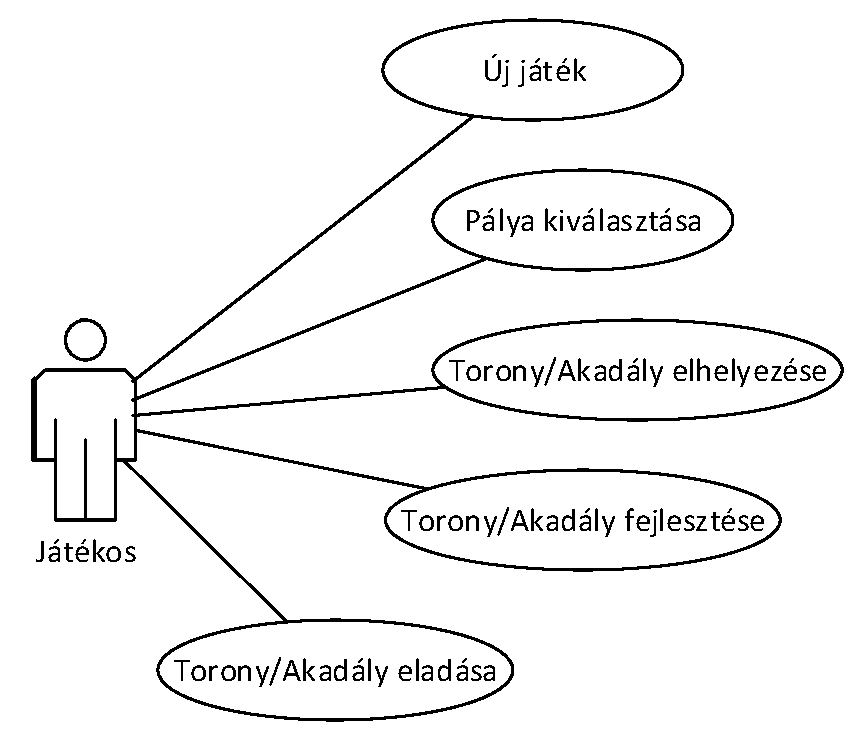
\includegraphics[width=17cm]{chapters/chapter02/images/2_4_2_use_case_diagram.eps}
\caption{Grafikus interfész}
\label{fig:Use-case_diagram}
\end{center}
\end{figure}


\section{Szótár}
\begin{description}

\item[akadály (obstacle)] az út celláira helyezett védelmi egység, a felette haladó ellenségek lassabban haladnak
\item[belépési pont (entry point)] az a hely, ahol az ellenségek belépnek a pályára
\item[cella (cell)] a pálya négyzetrácsos szerkezetét alkotó elemek
\item[eladás (sell)] egy védelmi egység megszűntetése, ami az arra költött varázserő egy részének visszatérülésével jár
\item[elhasználódás (attrition)] a csapdák amortizációja, amit a rajtuk áthaladó ellenségek okoznak
\item[elhelyezés (placing)] egy védelmi egység a pálya egy bizonyos cellájára való telepítése varázserőért cserébe
\item[ellenség (enemy)] azok az egységek, amik a pálya belépési pontjainál jönnek be, és a Végzet Hegye felé haladnak. Fajtái: tünde, törp, hobbit, ember
\item[ember(human)] az ellenség egy fajtája, sebessége közepes, életereje közepes
\item[életerő (health)] ellenségeket jellemző érték, amit a tornyokból kilőtt lövedékekkel lehet csökkenteni. Ha eléri a 0-t az ellenség meghal.
\item[faj: ellenség típusok] tünde, törp, hobbit, ember
\item[fejlesztés (upgrade)] egy védelmi egység hatékonyabbá tétele kristállyal
\item[gépigény] olyan számítógépes hardverek és nem hardveres erőforrások, amelyek minimálisan szükségesek a szoftver telepíthetőségéhez, rendes működéséhez
\item[háttér (background)] a pálya úton kívüli része, ide helyezhetjük a tornyokat
\item[hobbit(hobbit)] az ellenség egy fajtája, sebessége lassú, életereje alacsony
\item[játékos (player)] a szoftver felhasználója
\item[kristály (gem)] tornyok/akadályok fejlesztésére alkalmas varázseszköz
\item[kristály tartó(gem slot)] a tornyok kristályokat tároló helyei
\item[nyerni (win)] az akkor fennálló helyzet, mikor elfogynak az ellenségek, és egy sem jutott be a Végzet Hegyébe
\item[pálya (map)] játéktér, legalább 1 út van rajta, minden más része háttér
\item[readme] olyan fájl, amely információkat tartalmaz a szoftver telepítéséről és használatba vételéről
\item[sebez (damage)] csökkenti az ellenség életerejét
\item[szótár] ez a dokumentum
\item[torony (tower)] a háttér celláira helyezett védelmi egység, automatikusan tüzel az ellenségre
\item[törp(dwarf)] az ellenség egy fajtája, sebessége lassú, életereje magas
\item[tünde(elf)] az ellenség egy fajtája, sebessége gyors, életereje magas
\item[tüzel (fire)] lövedéket kibocsát, mellyel ellenséget sebez meg
\item[újratöltési idő(reload time)] a torony két tüzelése között eltelt idő
\item[út (way, road)] a pálya azon része, ahol az ellenséges egységek haladnak, és az akadályokat helyezhetjük
\item[varázserő (witchcraft)] a játékban használt fizetőeszköz, cserébe lehet a védelmi egységeket elhelyezni, fejleszteni
\item[védelmi egység] torony vagy akadály
\item[Végzet Hegye] az ellenségek célpontja, az ide való eljutásuk megakadályozása a játékos célja
\item[veszíteni (lose)] az akkor fennálló helyzet, mikor egy ellenség bejut a Végzet Hegyébe

\end{description}

%\comment{A szótár a követelmények alapján készítendő fejezet. Egy szótári bejegyzés definiálásához csak más szótári bejegyzések és köznapi – a feladattól független – fogalmak használhatók fel. A szótár mérete kb. 1-2 oldal legyen.}

\section{Projekt terv}
\subsection{Határidők}
\begin{longtable}{| l | l | l |}
\hline
\textbf{} & \textbf{Dátum} & \textbf{Feladat}
\tabularnewline
\hline


1 & febr. 14. & 14 h - csapatok regisztrációja \tabularnewline \hline
2 & febr. 24. & Követelmény, projekt, funkcionalitás - beadás \tabularnewline \hline
3 & márc. 3. & Analízis modell kidolgozása 1. - beadás \tabularnewline \hline
4 & márc. 10. & Analízis modell kidolgozása 2. - beadás \tabularnewline \hline
5 & márc. 17. & Szkeleton tervezése - beadás \tabularnewline \hline
6 & márc. 24. & Szkeleton - beadás \tabularnewline \hline
7 & márc. 31. & Prototípus koncepciója - beadás \tabularnewline \hline
8 & ápr. 7. & Részletes tervek - beadás \tabularnewline \hline
9 & ápr. 22. & Prototípus - beadás \tabularnewline \hline
10 & ápr. 28. & Grafikus felület specifikációja - beadás \tabularnewline \hline
11 & máj. 12. & Grafikus változat - beadás \tabularnewline \hline
12 & máj. 16. & Összefoglalás - beadás \tabularnewline \hline


\end{longtable}
\subsection{Átadás}

A szoftvert három fő fázisban adjuk át:
\paragraph{1.	Szkeleton}
A szoftver váza, az átadott részletes specifikáció, és analízis modell alapján. Ez a verzió csak a modell működését szemlélteti, csak karakteres ki- és bemenetekkel.

Az objektumoknak csak az interfésze definiált.

Az egyes metódusok, kiírják a képernyőre nevüket és meghívják azon metódusokat, amelyeket a szolgáltatás végrehajtása érdekében meg kell hívniuk. Elágazás esetén feltesz egy kérdést, aminek a válasza alapján fut tovább a modell.
\paragraph{2.	Prototípus}
Elkészült szoftver minden tulajdonságával bír a prototípus, csak a grafikus megjelenítés hiányzik róla. A pillanatnyi állapotot alfanumerikus képernyőn lehet követni, illetve log fájlokba menti a futásának részleteit.
\paragraph{3.	Grafikus változat}
A prototípustól csak a megjelenésben különbözik, illetve annak belső megvalósításával bővített változata.

\subsection{Szerepkörök}
\begin{itemize}


\item{Csapatvezető: Elekes Tamás}
\begin{itemize}
\item{Értekezlet előkészületei, lebonyolítása }
\item{Project felügyelet}
\item{Kód tervezés}
\item{Implementálás}
\item{Audio programozás}
\end{itemize}
\item{Fuksz Domonkos}
\begin{itemize}
\item{Dokumentálás}
\item{Dokumentumok formai minősége}
\item{Tesztelés}
\item{Kódolás}
\end{itemize}
\item{Nagy András}
\begin{itemize}
\item{Értekezletek logolása}
\item{Implementálás}
\item{Tesztelés}
\end{itemize}
\item{Seres Márk Dániel}
\begin{itemize}
\item{Feladat beadás}
\item{Implementálás}
\item{Tesztelés}
\item{UML diagram készítés}
\end{itemize}
\item{Rédey Bálint}
\begin{itemize}
\item{Dokumentálás}
\item{Implementálás}
\item{Grafikus programozás}
\item{UML diagram készítés}
\item{Feladatok feltöltése}
\end{itemize}
\end{itemize}

Ezen felül minden csapattagnak a konzultációkat látogatnia kell, illetve heti 1 teljes létszámú értekezleten részt kell vennie.
\subsection{Felhasznált fejlesztőeszközök}
\begin{description}
\item[Verziókezelés] A csoportmunka szempontjából nagyon fontos, hogy mindenki naprakészen hozzáférjen a kód és a dokumentumok aktuális verzióihoz. Ehhez a Git verziókezelő rendszert választottuk, ami felhő alapú, könnyen kezelhető rendszer.

\item[Java JDK] A szoftvert Java nyelven kerül implementálásra, amihez az ingyenes Eclipse szoftvert használjuk. Az Eclipse nagyon jó környezetet ad Java JUnit tesztelés végzésére is.

\item[UML] Fontos a jó minőségű dokumentáció elkészítéséhez az ábrák megfelelő és szép elkészítése. Erre a célra több UML rajzoló szoftvert is használunk: StarUML és Microsoft Office Visio 2013.

\item[Kommunikáció] A csapatmunka során elengedhetetlen a megfelelő kommunikáció a tagok között. Egyszerű szöveges kommunikációra Facebook csoportot használunk, míg fontosabb dolgok tárgyalásakor a Skype konferenciabeszélgetést használjuk.
\end{description}
%\comment{Tartalmaznia kell a projekt végrehajtásának lépéseit, a lépések, eredmények határidejét, az egyes feladatok elvégzéséért felelős személyek nevét és beosztását, a szükséges erőforrásokat, stb. Meg kell adni a csoportmunkát támogató eszközöket, a választott technikákat! Definiálni kell, hogy hogyan történik a dokumentumok és a forráskód megosztása!}


